\documentclass[border=10pt]{standalone}
\usepackage[svgnames]{xcolor}
\usepackage{amsmath}
\usepackage{pgfplots}
\pgfplotsset{compat=newest}
\usepackage[sfdefault]{FiraSans}
\usepackage{FiraMono}
\renewcommand*\familydefault{\sfdefault}
\begin{document}
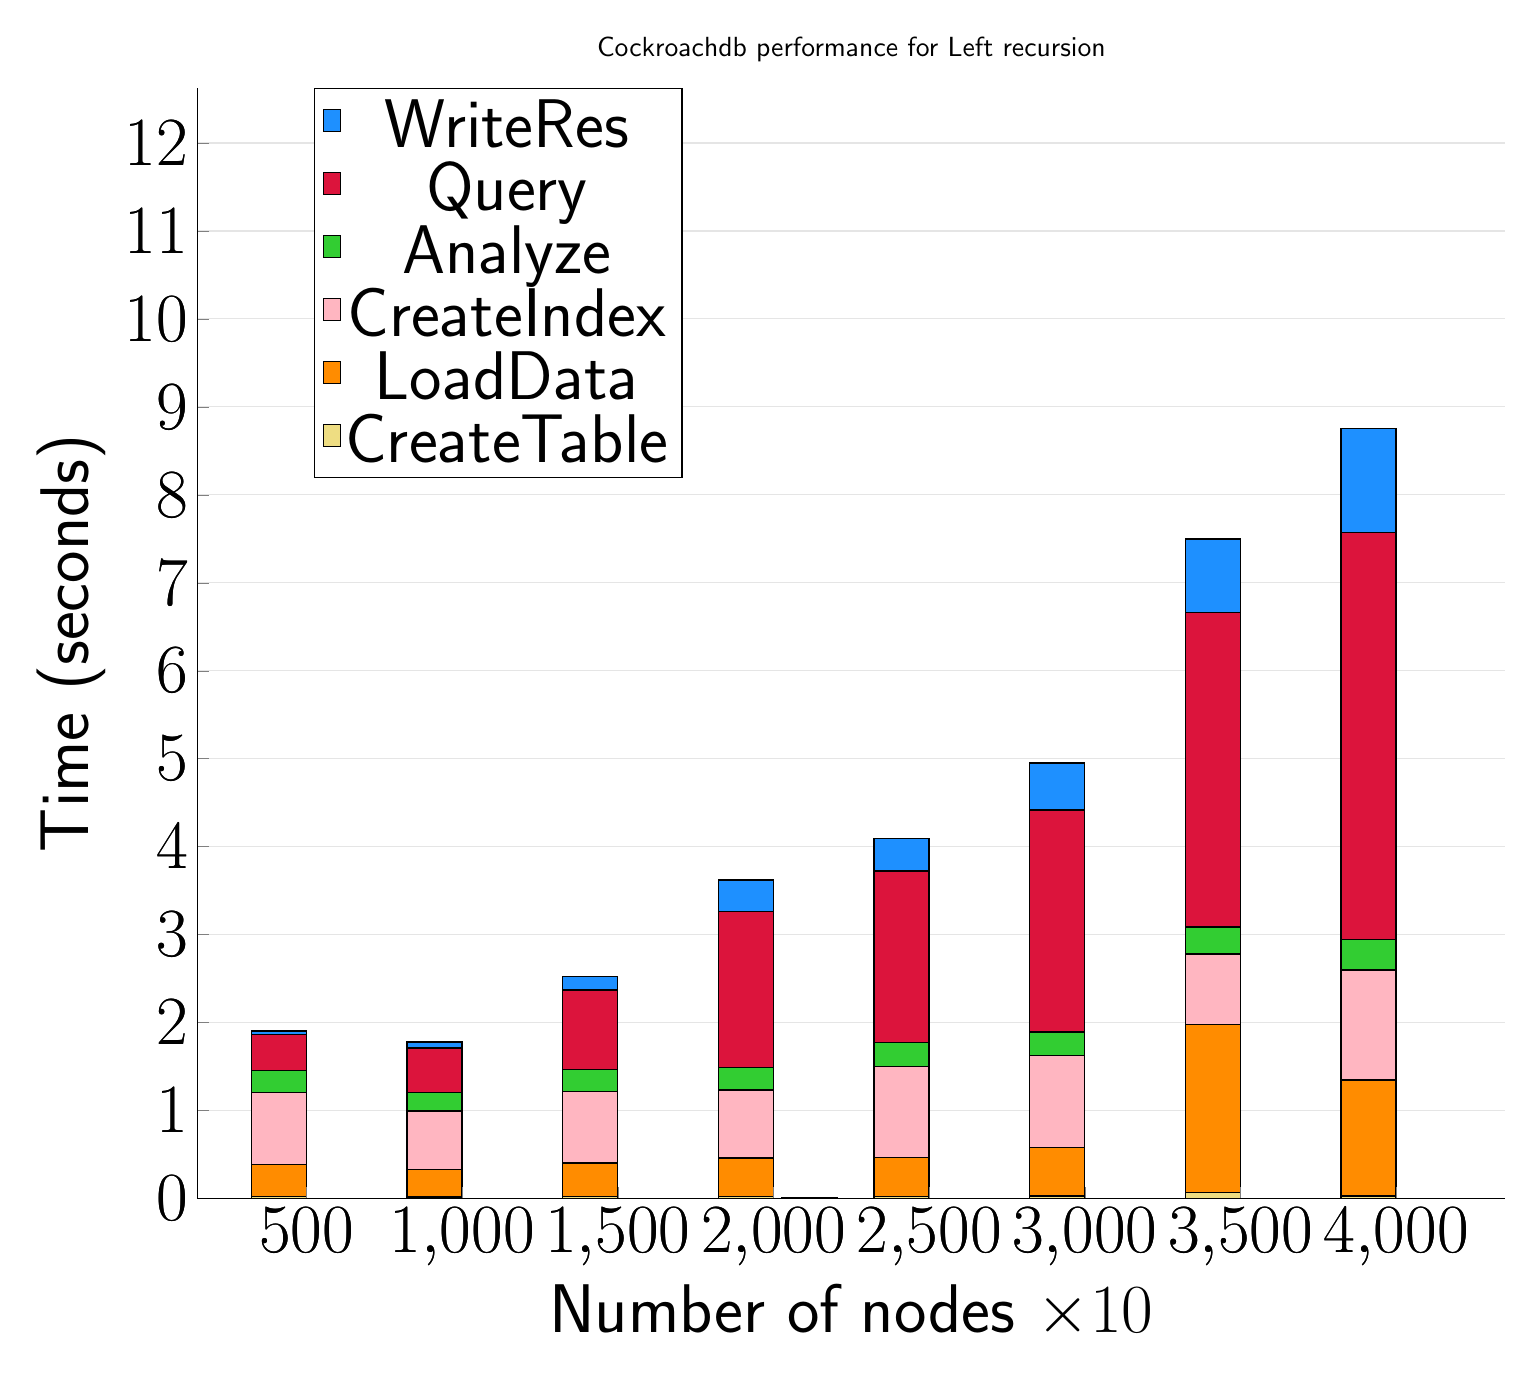
\begin{tikzpicture}
\begin{axis}[
   ybar stacked,
   title={Cockroachdb performance for Left recursion},
   bar shift=-10pt,
   width=1.5\textwidth,
   bar width=0.7cm,
   ymajorgrids, tick align=inside,
   major grid style={draw=gray!20},
   xtick=data,
   ymin=0, ymax=12.626666667560738,
   axis x line*=bottom,
   axis y line*=left,
   enlarge x limits=0.1,
   legend style={
       at={(0.23, 1)},
       anchor=north,
       legend columns=1,
       font=\Huge,
   },
   ylabel={Time (seconds)},
   xlabel={Number of nodes $\times 10$},
   label style={font=\Huge},
   tick label style={font=\Huge},
]
\addlegendimage{fill=DodgerBlue, draw=black, line width=0.2pt}
\addlegendentry{WriteRes}
\addlegendimage{fill=Crimson, draw=black, line width=0.2pt}
\addlegendentry{Query}
\addlegendimage{fill=LimeGreen, draw=black, line width=0.2pt}
\addlegendentry{Analyze}
\addlegendimage{fill=LightPink, draw=black, line width=0.2pt}
\addlegendentry{CreateIndex}
\addlegendimage{fill=DarkOrange, draw=black, line width=0.2pt}
\addlegendentry{LoadData}
\addlegendimage{fill=LightGoldenrod, draw=black, line width=0.2pt}
\addlegendentry{CreateTable}
\addplot +[fill=LightGoldenrod, draw=black, line width=0.5pt] coordinates {
    (500, 0.019999998311201733)
    (1000, 0.016666663189729054)
    (1500, 0.020000000794728596)
    (2000, 0.023333333432674408)
    (2500, 0.020000003278255463)
    (3000, 0.02999999870856603)
    (3500, 0.0700000027815501)
    (4000, 0.030000001192092896)
};
\addplot +[fill=DarkOrange, draw=black, line width=0.5pt] coordinates {
    (500, 0.36999999980131787)
    (1000, 0.3166666676600774)
    (1500, 0.38333333283662796)
    (2000, 0.4400000000993411)
    (2500, 0.4499999980131785)
    (3000, 0.5533333321412405)
    (3500, 1.9099999989072483)
    (4000, 1.3200000002980232)
};
\addplot +[fill=LightPink, draw=black, line width=0.5pt] coordinates {
    (500, 0.8133333325386047)
    (1000, 0.6600000013907751)
    (1500, 0.8133333325386047)
    (2000, 0.7699999983112017)
    (2500, 1.030000001192093)
    (3000, 1.0433333367109299)
    (3500, 0.7999999995032946)
    (4000, 1.2466666673620541)
};
\addplot +[fill=LimeGreen, draw=black, line width=0.5pt] coordinates {
    (500, 0.25333333512147266)
    (1000, 0.20999999592701593)
    (1500, 0.25333333512147266)
    (2000, 0.26000000288089115)
    (2500, 0.2733333334326744)
    (3000, 0.2666666656732559)
    (3500, 0.30666666726271313)
    (4000, 0.3500000014901161)
};
\addplot +[fill=Crimson, draw=black, line width=0.5pt] coordinates {
    (500, 0.40666666875282925)
    (1000, 0.5066666677594185)
    (1500, 0.8999999985098839)
    (2000, 1.7733333334326744)
    (2500, 1.9500000004967053)
    (3000, 2.5233333334326744)
    (3500, 3.573333332935969)
    (4000, 4.626666667560737)
};
\addplot +[fill=DodgerBlue, draw=black, line width=0.5pt] coordinates {
    (500, 0.03999999910593033)
    (1000, 0.07000000029802322)
    (1500, 0.15666666875282922)
    (2000, 0.35333333164453506)
    (2500, 0.36999999980131787)
    (3000, 0.5333333338300387)
    (3500, 0.8366666659712791)
    (4000, 1.1833333298563957)
};
\end{axis}
\begin{axis}[
   ybar stacked,
   bar shift=13pt,
   width=1.5\textwidth,
   bar width=0.7cm,
   ymajorgrids, tick align=inside,
   major grid style={draw=none},
   xtick=data,
   ymin=0, ymax=12.626666667560738,
   axis x line*=none,
   axis y line*=none,
   enlarge x limits=0.1,
   label style={font=\Huge},
   tick label style={font=\Huge},
]
\addplot +[fill=LightGoldenrod, draw=black, line width=0.5pt] coordinates {
    (500, 0.0)
    (1000, 0.0)
    (1500, 0.0)
    (2000, 0.0)
    (2500, 0.0)
    (3000, 0.0)
    (3500, 0.0)
    (4000, 0.0)
};
\addplot +[fill=DarkOrange, draw=black, line width=0.5pt] coordinates {
    (500, 0.003333333333333336)
    (1000, 0.0)
    (1500, 0.0)
    (2000, 0.0)
    (2500, 0.0)
    (3000, 0.0)
    (3500, 0.0033333333333333327)
    (4000, 0.0)
};
\addplot +[fill=LightPink, draw=black, line width=0.5pt] coordinates {
    (500, 0.0)
    (1000, 0.0)
    (1500, 0.0)
    (2000, 0.010000000000000007)
    (2500, 0.0)
    (3000, 0.0)
    (3500, 0.0)
    (4000, 0.0)
};
\addplot +[fill=LimeGreen, draw=black, line width=0.5pt] coordinates {
    (500, 0.0)
    (1000, 0.0)
    (1500, 0.0)
    (2000, 0.0)
    (2500, 0.0)
    (3000, 0.0)
    (3500, 0.0)
    (4000, 0.0)
};
\addplot +[fill=Crimson, draw=black, line width=0.5pt] coordinates {
    (500, 0.0)
    (1000, 0.0)
    (1500, 0.0)
    (2000, 0.0)
    (2500, 0.0)
    (3000, 0.0)
    (3500, 0.0)
    (4000, 0.0)
};
\addplot +[fill=DodgerBlue, draw=black, line width=0.5pt] coordinates {
    (500, 0.0)
    (1000, 0.0)
    (1500, 0.0)
    (2000, 0.0)
    (2500, 0.0)
    (3000, 0.0)
    (3500, 0.0)
    (4000, 0.0)
};
\end{axis}
\end{tikzpicture}

\end{document}
